Ο όρος ``ρομποτική κινητής βάσης" αναφέρεται σε ρομπότ τα οποία έχουν τη
δυνατότητα κίνησης στο περιβάλλον τους, σε αντίθεση με εκείνα των οποίων η βάση
είναι πακτωμένη σε μία συγκεκριμένη θέση του χώρου. Ως εκ τούτου η έρευνα αυτού
του τομέα ασχολείται με όλα εκείνα τα προβλήματα που απορρέουν από την πλοήγηση
ενός ρομπότ από μία θέση σε μία άλλη.


%%%%%%%%%%%%%%%%%%%%%%%%%%%%%%%%%%%%%%%%%%%%%%%%%%%%%%%%%%%%%%%%%%%%%%%%%%%%%%%%
\subsection{Θεμελιώδεις λειτουργίες}

Το πρόβλημα της πλοήγησης διακρίνεται σε βαθμούς αυτονομίας. Κάθε επόμενη
βαθμίδα αυτονομίας αφομοιώνει μία ανεξάρτητη μεταβλητή προηγούμενης βαθμίδας ως
μία προς υπολογισμό, την οποία εξαρτά από τον αρχικό στόχο. Η αυτονομία
πλοήγησης ξεκινάει από την τυχαία κίνηση στο χώρο με εντολές κίνησης
υπολογιζόμενες από το ρομπότ, στην παρακολούθηση προκαθορισμένων τροχιών,
ύστερα στην αυτόνομη χάραξη τροχιών προς προκαθορισμένους στόχους και την
αυτόνομη παρακολούθηση των τροχιών, και καταλήγει στην αυτόνομη πλοήγηση με
αυτόνομη επιλογή σημείων-στόχων.

Κοιτώντας την μη-τετριμμένη αυτόνομη πλοήγηση από το επίπεδο της επιφάνειας
απαιτείται κατ' ελάχιστον η γνώση δύο μεταβλητών: του στόχου προς τον οποίο το
ρομπότ θα κινηθεί και η τρέχουσα θέση του. Αυτές οι αθώες μεταβλητες ανοίγουν
την πόρτα σε ένα σύμπαν προβλημάτων μερικών από των οποίων τη λύση αποπειράται
η παρούσα διατριβή.

Για τον ακριβή προσδιορισμό ενός σημείου στο φυσικό χώρο απαιτείται αυτός ο
χώρος να φέρει σύστημα συντεταγμένων, και κατά συνέπεια να είναι μετρικός.
Έπειτα, με γνώμονα την ασφάλεια του ρομπότ και του περιβάλλοντός του, το ρομπότ
πρέπει να έχει γνώση των κατειλειμένων και μη σημείων από εμπόδια σε αυτό το
σύστημα. Από αυτές τις αιτίες προκύπτει η ανάγκη για την αναπαράσταση του
περιβάλλοντος με τη μορφή μετρικού χάρτη. Εν γένει το σύστημα συντεταγμένων και
ο χάρτης θα πρέπει να εφευρεθούν επί τούτου για κάθε περιβάλλον καθώς στη
γενική περίπτωση τα αρχιτεκτονικά σχέδια χώρων δεν είναι γνωστά. Από αυτή την
απαίτηση προκύπτει το πρόβλημα του SLAM (Simultaneous Localisation and
Mapping), δηλαδή της ταυτόχρονης κατασκευής χάρτη και εύρεσης της στάσης ενός
ρομποτ σε αυτόν.

Κατά συνέπεια η γνώση μιας οποιασδήποτε θέσης στο φυσικό χώρο μεσολαβείται από
τη γνώση της στο χάρτη του, στο οικείο του σύστημα αναφοράς. Δεδομένου του
χάρτη ενός χώρου ένα ρομπότ μπορεί να προσδιορίσει τη θέση του σε αυτόν
χρησιμοποιώντας τους αισθητήρες του, αντιπαραβάλλοντας μετρήσεις από αυτούς με
εικονικές μετρήσεις από κάποια υπόθεση-εκτίμηση για τη θέση του στο χάρτη. Το
πρόβλημα της έυρεσης της θέσης ενός ρομπότ στο χάρτη είναι θεμελιώδους
σημασίας στη ρομποτική κινητής βάσης, και διακρίνεται σε τριών ειδών προβλήματα
(σχήμα \ref{fig:localisation_problems_pie} \cite{Panigrahi2021}):

\begin{itemize}
  \item Εύρεση της θέσης βάσει καθολικής αβεβαιότητας (Global Localisation)
  \item Εύρεση και παρακολούθηση της θέσης βάσει περιορισμένης αβεβαιότητας (Pose Tracking)
  \item Ανίχνευση απαγωγής ρομπότ και εύρεση της νέας θέσης του (Kidnapped Robot Problem)
\end{itemize}

\begin{bw_box}
\begin{remark}
  Λόγω της παραδοχής \ref{ass:01_01} η θέση του ρομπότ δεν είναι μετρήσιμη
  αλλά παρατηρήσιμη.
  \label{remark:observable}
\end{remark}
\end{bw_box}

\begin{figure}\centering
  \vspace{-1cm}
  % GNUPLOT: LaTeX picture with Postscript
\begingroup
  \makeatletter
  \providecommand\color[2][]{%
    \GenericError{(gnuplot) \space\space\space\@spaces}{%
      Package color not loaded in conjunction with
      terminal option `colourtext'%
    }{See the gnuplot documentation for explanation.%
    }{Either use 'blacktext' in gnuplot or load the package
      color.sty in LaTeX.}%
    \renewcommand\color[2][]{}%
  }%
  \providecommand\includegraphics[2][]{%
    \GenericError{(gnuplot) \space\space\space\@spaces}{%
      Package graphicx or graphics not loaded%
    }{See the gnuplot documentation for explanation.%
    }{The gnuplot epslatex terminal needs graphicx.sty or graphics.sty.}%
    \renewcommand\includegraphics[2][]{}%
  }%
  \providecommand\rotatebox[2]{#2}%
  \@ifundefined{ifGPcolor}{%
    \newif\ifGPcolor
    \GPcolorfalse
  }{}%
  \@ifundefined{ifGPblacktext}{%
    \newif\ifGPblacktext
    \GPblacktexttrue
  }{}%
  % define a \g@addto@macro without @ in the name:
  \let\gplgaddtomacro\g@addto@macro
  % define empty templates for all commands taking text:
  \gdef\gplbacktext{}%
  \gdef\gplfronttext{}%
  \makeatother
  \ifGPblacktext
    % no textcolor at all
    \def\colorrgb#1{}%
    \def\colorgray#1{}%
  \else
    % gray or color?
    \ifGPcolor
      \def\colorrgb#1{\color[rgb]{#1}}%
      \def\colorgray#1{\color[gray]{#1}}%
      \expandafter\def\csname LTw\endcsname{\color{white}}%
      \expandafter\def\csname LTb\endcsname{\color{black}}%
      \expandafter\def\csname LTa\endcsname{\color{black}}%
      \expandafter\def\csname LT0\endcsname{\color[rgb]{1,0,0}}%
      \expandafter\def\csname LT1\endcsname{\color[rgb]{0,1,0}}%
      \expandafter\def\csname LT2\endcsname{\color[rgb]{0,0,1}}%
      \expandafter\def\csname LT3\endcsname{\color[rgb]{1,0,1}}%
      \expandafter\def\csname LT4\endcsname{\color[rgb]{0,1,1}}%
      \expandafter\def\csname LT5\endcsname{\color[rgb]{1,1,0}}%
      \expandafter\def\csname LT6\endcsname{\color[rgb]{0,0,0}}%
      \expandafter\def\csname LT7\endcsname{\color[rgb]{1,0.3,0}}%
      \expandafter\def\csname LT8\endcsname{\color[rgb]{0.5,0.5,0.5}}%
    \else
      % gray
      \def\colorrgb#1{\color{black}}%
      \def\colorgray#1{\color[gray]{#1}}%
      \expandafter\def\csname LTw\endcsname{\color{white}}%
      \expandafter\def\csname LTb\endcsname{\color{black}}%
      \expandafter\def\csname LTa\endcsname{\color{black}}%
      \expandafter\def\csname LT0\endcsname{\color{black}}%
      \expandafter\def\csname LT1\endcsname{\color{black}}%
      \expandafter\def\csname LT2\endcsname{\color{black}}%
      \expandafter\def\csname LT3\endcsname{\color{black}}%
      \expandafter\def\csname LT4\endcsname{\color{black}}%
      \expandafter\def\csname LT5\endcsname{\color{black}}%
      \expandafter\def\csname LT6\endcsname{\color{black}}%
      \expandafter\def\csname LT7\endcsname{\color{black}}%
      \expandafter\def\csname LT8\endcsname{\color{black}}%
    \fi
  \fi
    \setlength{\unitlength}{0.0500bp}%
    \ifx\gptboxheight\undefined%
      \newlength{\gptboxheight}%
      \newlength{\gptboxwidth}%
      \newsavebox{\gptboxtext}%
    \fi%
    \setlength{\fboxrule}{0.5pt}%
    \setlength{\fboxsep}{1pt}%
\begin{picture}(6000.00,6000.00)%
    \gplgaddtomacro\gplbacktext{%
    }%
    \gplgaddtomacro\gplfronttext{%
      \colorrgb{0.00,0.00,0.00}%
      \put(310,4777){\makebox(0,0)[l]{\strut{}Απαχθέν ρομπότ}}%
      \colorrgb{0.00,0.00,0.00}%
      \put(310,4457){\makebox(0,0)[l]{\strut{}Βάσει καθολικής αβεβαιότητας}}%
      \colorrgb{0.00,0.00,0.00}%
      \put(310,4137){\makebox(0,0)[l]{\strut{}Βάσει περιορισμένης αβεβαιότητας}}%
      \colorrgb{0.00,0.00,0.00}%
      \put(2120,3766){\makebox(0,0)[r]{\strut{}$19\%$}}%
      \put(1603,1878){\makebox(0,0)[r]{\strut{}$26\%$}}%
      \put(4455,2284){\makebox(0,0)[l]{\strut{}$55\%$}}%
    }%
    \put(0,0){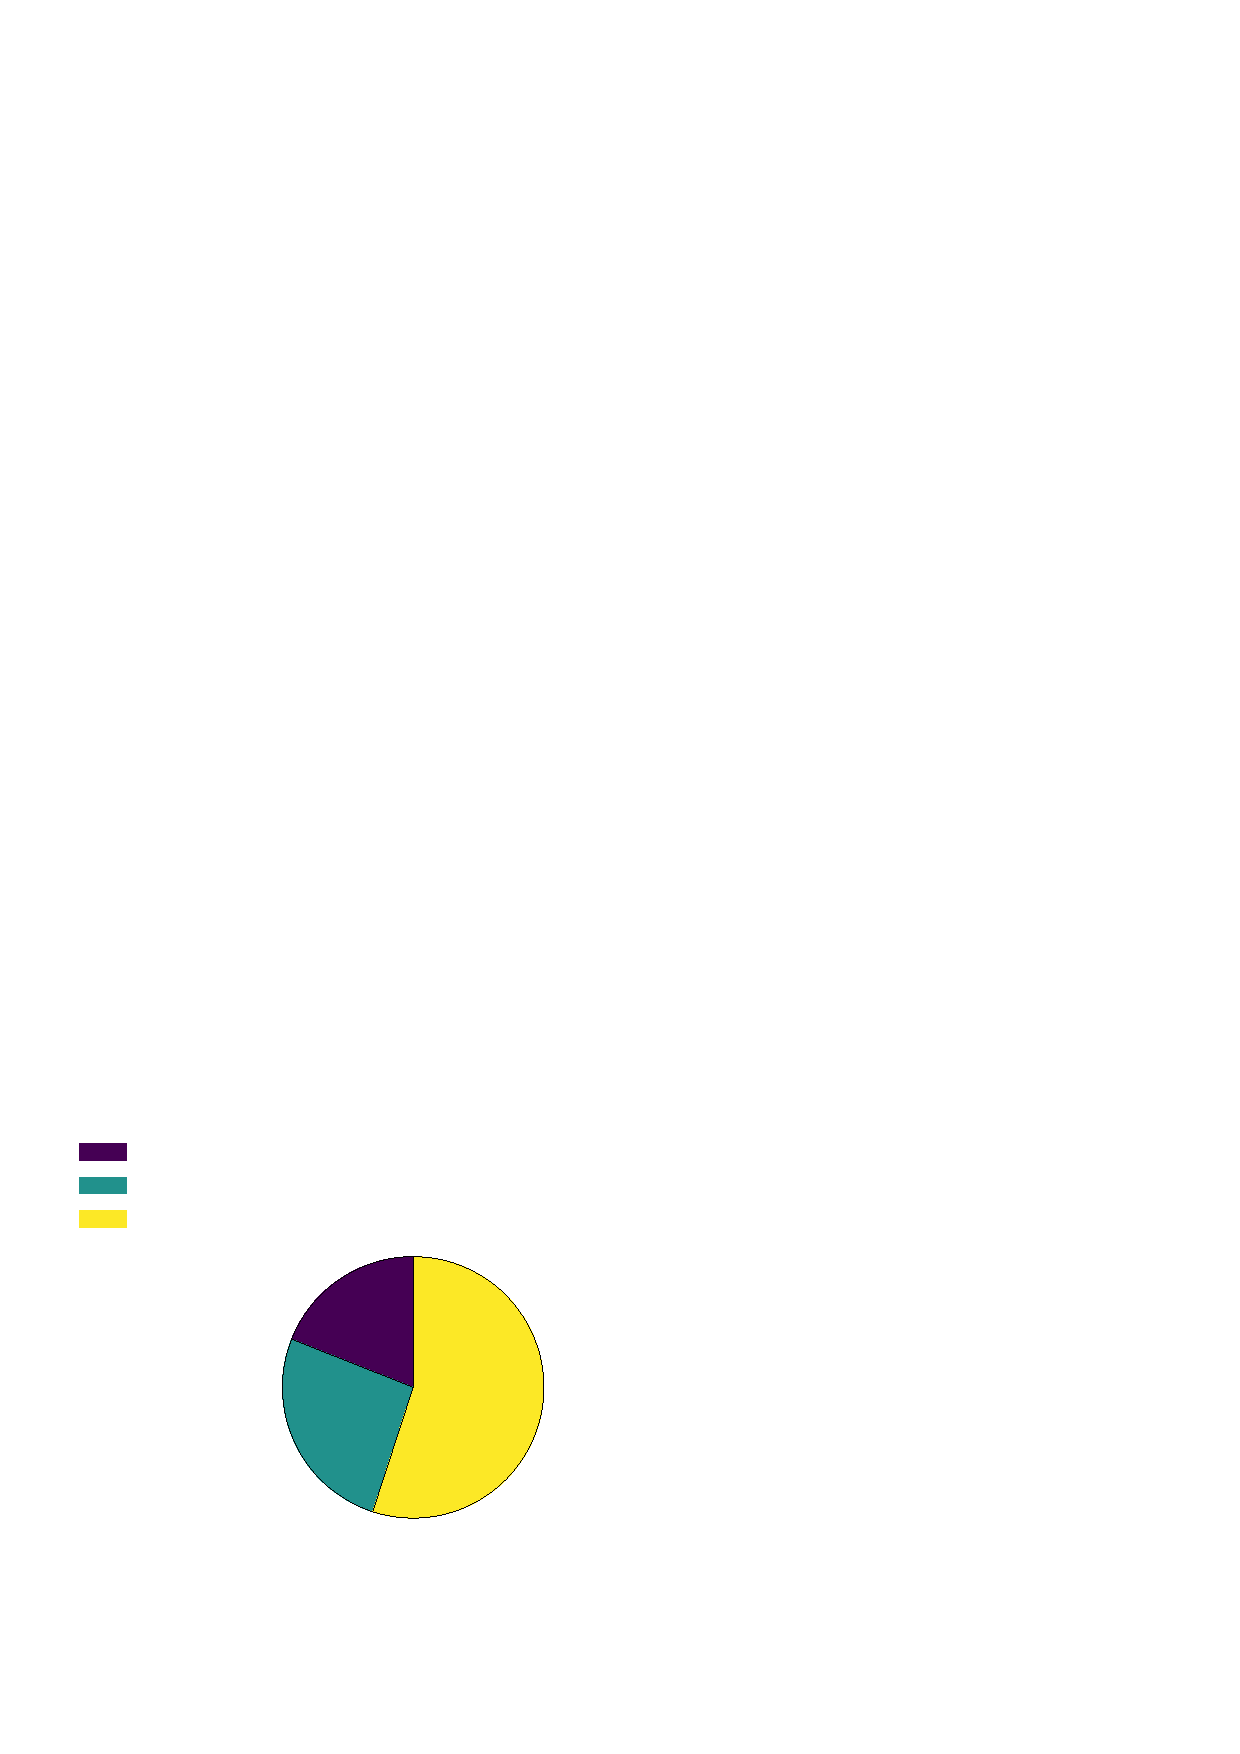
\includegraphics{./figures/parts/01/chapters/01/sections/01/localisation_problems_pie}}%
    \gplfronttext
  \end{picture}%
\endgroup

  \vspace{-2cm}
  \caption{\small Κατάτμηση του προβλήματος της εύρεσης θέσης σε κατηγορίες και
           τα ποσοστά έρευνας σε αυτές}
  \label{fig:localisation_problems_pie}
\end{figure}

Στο μεγαλύτερό της μέρος η παρούσα διατριβή εστιάζει στα δύο πρώτα προβλήματα,
των οποίων η λύση απαιτείται στην πράξη σε κάθε σύστημα με πεδίο εφαρμογής
\ref{scope} που ικανοποιεί την παραδοχή \ref{ass:01_01}.

Δεδομένης της γνώσης του χάρτη του περιβάλλοντος στο οποίο κινείται ένα ρομπότ
κινητής βάσης, της αρχικής και της επιθυμητής του θέσης, ενός αλγορίθμου
παρακολούθησης της θέσης του (pose tracking), και αισθητήρων για την αντίληψη
του περιβάλλοντος, στη γενικότερή του μορφή το πρόβλημα της αυτόνομης πλοήγησης
είναι επιλύσιμο. Για την επίλυσή του απαιτούνται δύο μέθοδοι:

\begin{itemize}
  \item Ένας αλγόριθμος χάραξης μονοπατιού που συνδέει την αρχική με την τελική
        του θέση (Path Planning)
  \item Ένας ελεγκτής κίνησης του ρομπότ για την παρακολούθηση του παραπάνω
        μονοπατιού (Motion Controller)
\end{itemize}


%%%%%%%%%%%%%%%%%%%%%%%%%%%%%%%%%%%%%%%%%%%%%%%%%%%%%%%%%%%%%%%%%%%%%%%%%%%%%%%%
\subsection{Πηγές και τρόποι αντίληψης του περιβάλλοντος}

Η επιτυχής λύση του προβλήματος της αυτόνομης πλοήγησης προϋποθέτει την ύπαρξη
και χρήση εξωδεκτικών αισθητήρων. Χωρίς αυτούς τα προβλήματα των οποίων η λύση
είναι αναγκαία για την αυτόνομη πλοήγηση (κατασκευή χάρτη, εύρεση και
παρακολούθηση της θέσης του ρομπότ) δεν είναι επιλύσιμα. Για την αντίληψη των
ορίων (επιφάνειες εμπόδια) του περιβάλλοντος χρησιμοποιούνται αισθητήρες με
ποικίλα χαρακτηριστικά, ανάλογα με τα χαρακτηριστικά του περιβάλλοντος και
την αντικειμενική επιδίωξη της χρήσης ρομπότ κινητής βάσης. Όσο τα χρόνια
περνούσαν και η τεχνολογία υλικών εκλεπτυνόταν, μαζί της εξελίσσονταν και
οι παραπάνω αλγόριθμοι, οξύνοντας την ακρίβεια εκτίμησης της αναπαράστασης
του περιβάλλοντος χώρου και της θέσης ενός ρομπότ σε αυτό.

Τα πρώτα χρόνια της ρομποτικής χρησιμοποιούνταν αισθητήρες υπερήχων (sonar),
εκκινώντας από την ανίχνευση εμποδίων στη γειτονιά ενός ρομπότ. Η τεχνολογία
ήταν εκεί λόγω εκτεταμένης χρήσης τους σε στρατιωτικές επιχειρήσεις, και το
κόστος τους ήταν χαμηλό. Η αρχή λειτουργίας τους βασίζεται στην εκτίμηση
αποστάσεων προς τα γύρω εμπόδια μέσω της μέτρησης του χρόνου εκπομπής υπερήχων
προς και ανάκλασης από αυτά. Αν και χρησιμοποιούνται μέχρι και σήμερα, η χρήση
τους περιορίζεται στην ανίχνευση αντικειμένων σε χαμηλές αποστάσεις λόγω της
αδρής λεπτομέρειας των μετρήσεών τους, το περιορισμένο τους γωνιακό πεδίο
όρασης, και το εγγενές πρόβλημα της αμφισημίας των μετρήσεών τους λόγω των
πολλαπλών διαδοχικών ενδεχόμενων ανακλάσεων του ήχου σε επιφάνειες κλειστών
χώρων.

Την ίδια αρχή λειτουργίας εκμεταλλεύονται οι αισθητήρες lidar (σύντμηση του
Light και Radar) χρησιμοποιώντας, αντί για ήχο, φως υπέρυθρης, ορατής, ή
υπεριώδους ακτινοβολίας. Οι αισθητήρες LIDAR υστερούν σε κόστος, μέγεθος, και
συχνότητα μετρήσεων, αλλά εμφανίζουν σημαντικά μεγαλύτερο εύρος όρασης, τόσο
γωνιακά όσο και ακτινικά, και ακρίβεια μετρήσεων που μπορεί να φτάσει την τάξη
των μερικών εκατοστών. Η διαφορά της ακρίβειάς των μετρήσεών τους ως προς την
κατασκευή χάρτη με τη χρήση τους αποτυπώνεται στο σχήμα
\ref{fig:sonar_lidar_map}.

\begin{figure}\centering
  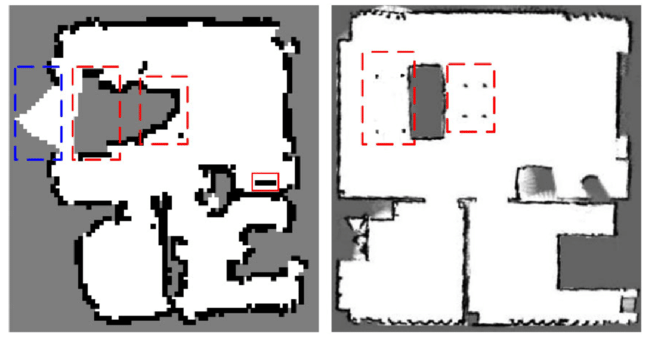
\includegraphics[scale=0.5]{./figures/01.01.mobile_robotics/sonar_lidar_map.png}
  \caption{\small Αριστερά: δισδιάστατος χάρτης από μετρήσεις αισθητήρα τύπου sonar.
           Δεξιά: χάρτης του ίδιου χώρου από μετρήσεις αισθητήρα τύπου lidar
           \cite{Qi2020}. Τα χρωματισμένα περιγράμματα περικλείουν περιοχές τις
           οποίες ο αισθητήρας sonar απέτυχε να χαρτογραφήσει με πιστότητα προς
           το πραγματικό περιβάλλον}
  \label{fig:sonar_lidar_map}
\end{figure}

Η ανάπτυξη της τεχνολογίας αισθητήρων εικόνας και η βελτίωση της ποιότητάς τους
τούς κατέστησε και πηγές εξωδεκτικών μετρήσεων στη ρομποτική. Το σημαντικό
τους προτέρημα είναι η χρωματική πληροφορία του περιβάλλοντος, το μεγάλο
οριζόντιο και κάθετο εύρος όρασής τους, και ο υψηλός ρυθμός ανανέωσης των
μετρήσεών τους. Στον αντίποδα, λόγω του μεγάλου όγκου πληροφορίας που φέρουν,
απαιτούν αντίστοιχους υπολογιστικούς πόρους, οι οποίοι στα πλαίσια του πεδίου
εφαρμογής \ref{scope} ενδέχεται να μην είναι διαθέσιμοι. Η εφεύρεση των
αισθητήρων εικόνας και βάθους (RGBD, ή η χρήση στερεοειδών συστημάτων) εισάγει
την επιπρόσθετη πληροφορία κατάληψης σημείων στον τρισδιάστατο χώρο από
εμπόδια, αλλά ταυτόχρονα επιφέρει χαμηλότερες συχνότητες ανανέωσης
αξιοποιήσιμης πληροφορίας λόγω του αυξημένου όγκου της χωρικής πλέον
πληροφορίας. Σε αντίθεση με τους προηγούμενους αισθητήρες εξαρτώνται από τις
συνθήκες φωτισμού του χώρου στον οποίον λειτουργούν και συνεπώς η ποιότητα των
μετρήσεων είναι ευμετάβλητη. Σε σχέση με τους αισθητήρες lidar εμφανίζουν
σημαντικά περιορισμένο γωνιακό εύρος όρασης, ακρίβεια μετρήσεων που φθίνει
τετραγωνικά σε σχέση με την απόσταση μέτρησης (αντί για γραμμικά όπως στους
αισθητήρες lidar), και περιοχές μη αξιοποιήσιμων μετρήσεων λόγω σκιών που
παράγονται ως συνέπεια της αρχής λειτουργίας τους \cite{Mallick2014}. Η διαφορά
της ακρίβειάς των μετρήσεών τους ως προς την κατασκευή χάρτη με τη χρήση τους
αποτυπώνεται στο σχήμα \ref{fig:rgbd_lidar_map}.

\begin{figure}\centering
  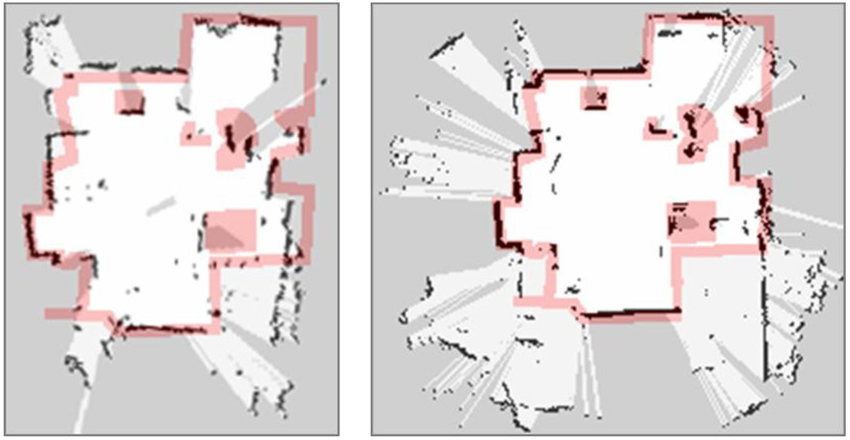
\includegraphics[scale=0.5]{./figures/01.01.mobile_robotics/rgbd_lidar_map.png}
  \caption{\small Αριστερά: δισδιάστατος χάρτης από μετρήσεις αισθητήρα τύπου RGBD.
           Δεξιά: χάρτης του ίδιου χώρου από μετρήσεις αισθητήρα τύπου lidar
           \cite{Oliver2012}. Οι κόκκινες γραμμές αναπαραστούν το πραγματικό
           περιβάλλον}
  \label{fig:rgbd_lidar_map}
\end{figure}



%\begin{bw_box}
%\begin{assumption}
  %\label{ass:01_01_01}
%\end{assumption}
%\end{bw_box}




%%%%%%%%%%%%%%%%%%%%%%%%%%%%%%%%%%%%%%%%%%%%%%%%%%%%%%%%%%%%%%%%%%%%%%%%%%%%%%%%
\subsection{Σύντομη Ιστορία}

%%%%%%%%%%%%%%%%%%%%%%%%%%%%%%%%%%%%%%%%%%%%%%%%%%%%%%%%%%%%%%%%%%%%%%%%%%%%%%%%
\subsection{Τρέχουσα κατάσταση}
